\documentclass[tikz,border=5pt]{standalone}
\usepackage[T1]{fontenc}
\usepackage{lmodern,amsmath,amssymb}
\usetikzlibrary{arrows.meta,calc,positioning,fit,backgrounds,shapes.geometric,matrix,decorations.pathreplacing,patterns}
\definecolor{ink}{gray}{0.08}
\definecolor{wash}{gray}{0.965}
\definecolor{soft}{gray}{0.45}
\tikzset{box/.style={draw=ink,line width=.65pt,fill=white,align=center,inner sep=4pt,outer sep=0pt,font=\small},flow/.style={draw=ink,line width=.65pt,-{Latex[length=1.8mm,width=1.3mm]},rounded corners=2pt},annotation/.style={font=\scriptsize,text=soft,align=center},groupbox/.style={draw=soft,dashed,line width=.45pt,fill=wash}}
\begin{document}
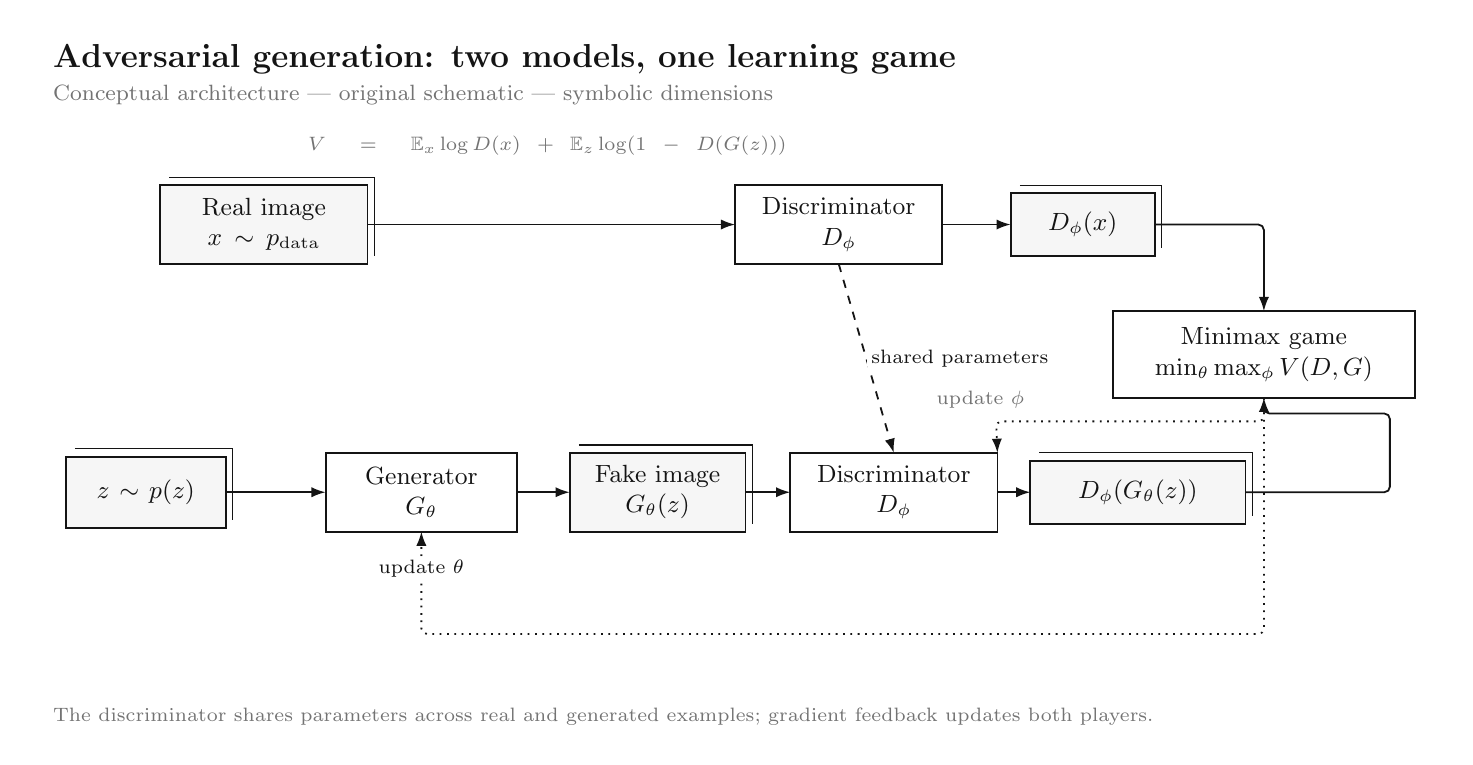
\begin{tikzpicture}[x=1cm,y=-1cm,font=\rmfamily,text=ink]

\path[use as bounding box] (0,0) rectangle (18,9);
\node[anchor=west,font=\large\bfseries] at (.2,.4) {Adversarial generation: two models, one learning game};
\node[anchor=west,font=\footnotesize,text=soft] at (.2,.85) {Conceptual architecture | original schematic | symbolic dimensions};
\begin{pgfonlayer}{background}
\end{pgfonlayer}
\node[box,fill=wash,minimum width=2.6cm,minimum height=1.0cm,text width=2.35cm] (real) at (3.0,2.5) {Real image\\$x\sim p_{\rm data}$};
\draw[ink,line width=.4pt] (1.8,1.9) -- (4.3999999999999995,1.9) -- (4.3999999999999995,2.9);
\node[box,minimum width=2.6cm,minimum height=1.0cm,text width=2.35cm] (dr) at (10.3,2.5) {Discriminator\\$D_\phi$};
\node[box,fill=wash,minimum width=1.8cm,minimum height=0.8cm,text width=1.55cm] (sr) at (13.4,2.5) {$D_\phi(x)$};
\draw[ink,line width=.4pt] (12.6,2.0) -- (14.4,2.0) -- (14.4,2.8);
\node[box,fill=wash,minimum width=2.0cm,minimum height=0.9cm,text width=1.75cm] (z) at (1.5,5.9) {$z\sim p(z)$};
\draw[ink,line width=.4pt] (0.6,5.3500000000000005) -- (2.6,5.3500000000000005) -- (2.6,6.250000000000001);
\node[box,minimum width=2.4cm,minimum height=1.0cm,text width=2.15cm] (g) at (5.0,5.9) {Generator\\$G_\theta$};
\node[box,fill=wash,minimum width=2.2cm,minimum height=1.0cm,text width=1.9500000000000002cm] (fake) at (8.0,5.9) {Fake image\\$G_\theta(z)$};
\draw[ink,line width=.4pt] (7.0,5.300000000000001) -- (9.2,5.300000000000001) -- (9.2,6.300000000000001);
\node[box,minimum width=2.6cm,minimum height=1.0cm,text width=2.35cm] (df) at (11.0,5.9) {Discriminator\\$D_\phi$};
\node[box,fill=wash,minimum width=2.7cm,minimum height=0.8cm,text width=2.45cm] (sf) at (14.1,5.9) {$D_\phi(G_\theta(z))$};
\draw[ink,line width=.4pt] (12.85,5.4) -- (15.549999999999999,5.4) -- (15.549999999999999,6.200000000000001);
\node[box,minimum width=3.8cm,minimum height=1.1cm,text width=3.55cm] (obj) at (15.7,4.15) {Minimax game\\$\min_\theta\max_\phi V(D,G)$};
\begin{pgfonlayer}{background}
\draw[flow] (real.east) -- (dr.west);
\draw[flow] (dr.east) -- (sr.west);
\draw[flow] (z.east) -- (g.west);
\draw[flow] (g.east) -- (fake.west);
\draw[flow] (fake.east) -- (df.west);
\draw[flow] (df.east) -- (sf.west);
\draw[flow] (sr.east) -- (15.7,2.5) -- (obj.north);
\draw[flow] (sf.east) -- (17.3,5.9) -- (17.3,4.9) -- (15.7,4.9) -- (obj.south);
\draw[flow,dashed] (dr.south) -- (df.north) node[midway,right,fill=white,inner sep=1.5pt,font=\scriptsize] {shared parameters};
\draw[flow,dotted] (obj.south) -- (15.7,5.0) -- (12.3,5.0) -- (df.north east);
\draw[flow,dotted] (obj.south) -- (15.7,7.7) -- (5,7.7) -- (g.south) node[midway,above,fill=white,inner sep=1.5pt,font=\scriptsize] {update $\theta$};
\end{pgfonlayer}
\node[annotation,text width=2.0cm] at (12.1,4.72) {update $\phi$};
\node[annotation,text width=11cm] at (6.6,1.5) {$V=\mathbb E_x\log D(x)+\mathbb E_z\log(1-D(G(z)))$};
\node[anchor=west,align=left,font=\scriptsize,text=soft,text width=17.6cm] at (.2,8.75) {The discriminator shares parameters across real and generated examples; gradient feedback updates both players.};
\end{tikzpicture}
\end{document}
